% !TEX TS-program = pdflatex
% !TEX encoding = UTF-8 Unicode

% This is a simple template for a LaTeX document using the "article" class.
% See "book", "report", "letter" for other types of document.

\documentclass[11pt]{article} % use larger type; default would be 10pt

\usepackage[utf8]{inputenc} % set input encoding (not needed with XeLaTeX)

%%% Examples of Article customizations
% These packages are optional, depending whether you want the features they provide.
% See the LaTeX Companion or other references for full information.

%%% PAGE DIMENSIONS
\usepackage{geometry} % to change the page dimensions
\geometry{letterpaper} % or letterpaper (US) or a5paper or....
\geometry{margin=1in} % for example, change the margins to 2 inches all round
% \geometry{landscape} % set up the page for landscape
%   read geometry.pdf for detailed page layout information

\usepackage{graphicx} % support the \includegraphics command and options
\usepackage{colortbl}
% \usepackage[parfill]{parskip} % Activate to begin paragraphs with an empty line rather than an indent
\usepackage{amssymb}
\usepackage{amsmath}
\usepackage{amsfonts}
\usepackage{bbm}
\usepackage{amsthm}

%%% PACKAGES
\usepackage{booktabs} % for much better looking tables
\usepackage{array} % for better arrays (eg matrices) in maths
\usepackage{paralist} % very flexible & customisable lists (eg. enumerate/itemize, etc.)
\usepackage{verbatim} % adds environment for commenting out blocks of text & for better verbatim
\usepackage{subfig} % make it possible to include more than one captioned figure/table in a single float
% These packages are all incorporated in the memoir class to one degree or another...

%%% HEADERS & FOOTERS
\usepackage{fancyhdr} % This should be set AFTER setting up the page geometry
\pagestyle{fancy} % options: empty , plain , fancy
\renewcommand{\headrulewidth}{0pt} % customise the layout...
\lhead{}\chead{}\rhead{}
\lfoot{}\cfoot{\thepage}\rfoot{}

%%% SECTION TITLE APPEARANCE
\usepackage{sectsty}
\allsectionsfont{\sffamily\mdseries\upshape} % (See the fntguide.pdf for font help)
% (This matches ConTeXt defaults)

%%% ToC (table of contents) APPEARANCE
\usepackage[nottoc,notlof,notlot]{tocbibind} % Put the bibliography in the ToC
\usepackage[titles,subfigure]{tocloft} % Alter the style of the Table of Contents
\usepackage{bbm}
\usepackage{endnotes}
\renewcommand{\qed}{\hfill\blacksquare}
\renewcommand{\cftsecfont}{\rmfamily\mdseries\upshape}
\renewcommand{\cftsecpagefont}{\rmfamily\mdseries\upshape} % No bold!
\DeclareMathOperator*{\argmax}{arg\,max}
\DeclareMathOperator*{\argmin}{arg\,min}
\usepackage{graphicx}
\graphicspath{ {./pings/} }

\newcount\colveccount
\newcommand*\colvec[1]{
	\global\colveccount#1
	\begin{pmatrix}
		\colvecnext
	}
	\def\colvecnext#1{
		#1
		\global\advance\colveccount-1
		\ifnum\colveccount>0
		\\
		\expandafter\colvecnext
		\else
	\end{pmatrix}
	\fi
}

\newcommand{\norm}[1]{\left\lVert#1\right\rVert}

\title{Problem Set \#4\\ ~\\ \large{Econ 899, Fall 2021} }
\author{Heejin Yoon}


\begin{document}
\maketitle
~\\

\section*{Exercise 1}
\begin{itemize}
	\item[1.] Stationary equilibrium results with social security ($\theta^{SS}_{0}=0.11$) and without it ($\theta^{SS}_{N}=0$) are presented below.
	
	\begin{center}
		\begin{tabular}{c|r|r} 
			\hline
			& \multicolumn{1}{c|}{With Social Security} & \multicolumn{1}{c}{Without Social Security}  \\ 
			\hline
			\textit{K}  & 3.361                                     & 4.624                                        \\
			\textit{L}  & 0.343                                     & 0.366                                        \\
			\textit{w}  & 1.456                                     & 1.600                                        \\
			\textit{r}  & 0.023                                     & 0.011                                        \\
			\textit{b}  & 0.226                                     & 0.000                                        \\
			\textit{W}  & -35.8                                     & -37.3                                        \\
			\textit{CV} & 0.598                                     & 0.673                                        \\
			\hline
		\end{tabular}
	\end{center}
	~\\~\\~
	\item[2.] Transition paths of interest rate, wage, capital, and effective labor are plotted in the following four figures. Since social security benefit is removed, the interest rate will instantly surge as the money need will increase from those who were previously able to receive social security benefits. Also, people will work more to insure their future lives by themselves, and a higher labor supply will immediately cut the wage level. Then as time passes by, a higher interest rate will gradually increase aggregate capital stock, and an increase in capital supply will reduce the interest rate. Also, lowered wages will make people gradually work less, and decreasing labor supply will make wages go up further. Overall, interest rate, wage, capital, and labor will converge into the new steady-state level.
	\pagebreak
	
		\begin{figure}[h]
			\centering
			\subfloat{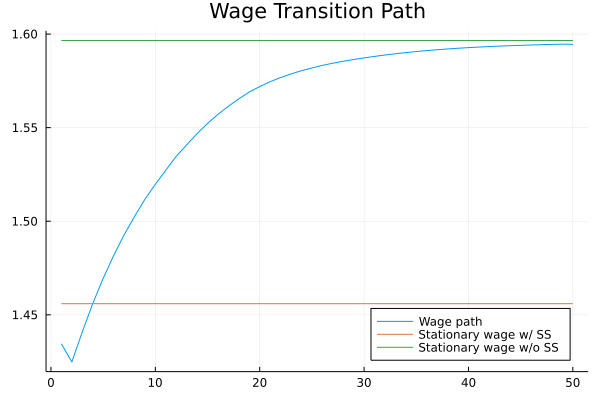
\includegraphics[width=.4\linewidth]{./julia/wage_path.png}}
			\subfloat{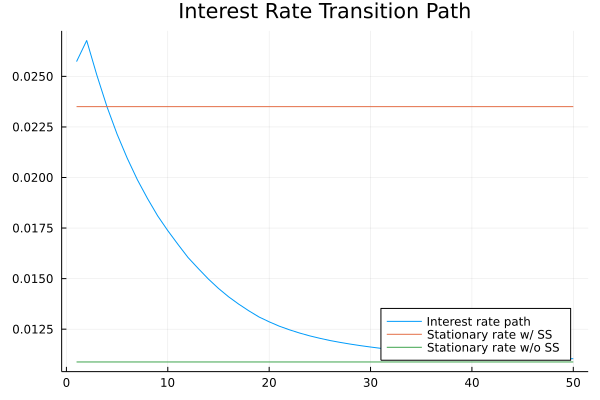
\includegraphics[width=.4\linewidth]{./julia/interest_rate_path.png}}
		\end{figure}

		\begin{figure}[h]
			\centering
			\subfloat{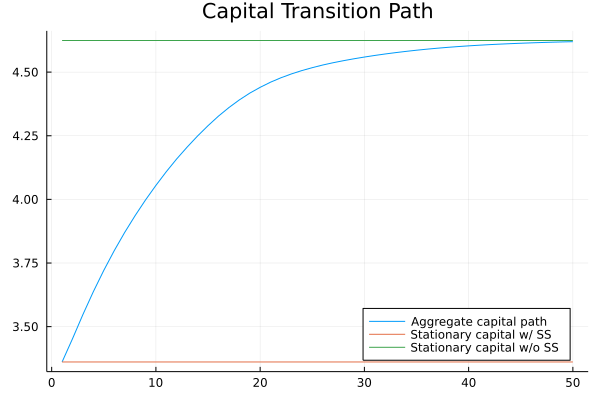
\includegraphics[width=.4\linewidth]{./julia/aggregate_capital_path.png}}
			\subfloat{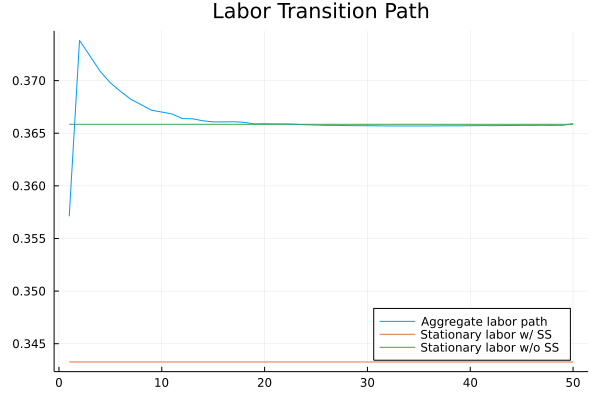
\includegraphics[width=.4\linewidth]{./julia/aggregate_labor_path.png}}
		\end{figure}
	
	~\\
	\item[3.] By calculating the consumption equivalent variation ($EV$) for each age, asset, and productivity shock grid and by summing up the measure of people whose $EV$ is greater or equal to $1$, we can see that $11.4\%$ of population will be better off by the reform. Thus, these people will support this change.
	
	The values of $EV$s by ages are plotted below. $EV$ decreases in age, as the elder have not accumulated enough funds for their life after the retirement.  
	
	\begin{center}
		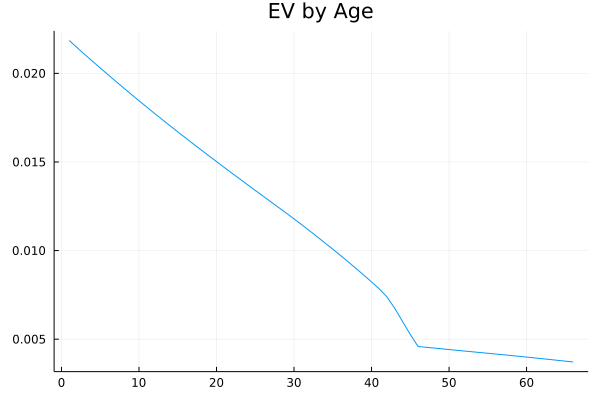
\includegraphics[width=.5\linewidth]{./julia/EV.png}
	\end{center}
\end{itemize}

\pagebreak

\section*{Exercise 2}
\begin{itemize}
	\item[1.] We can repeat the same analyses as Exercise 1, only making a change on the policy implementation time to $t=21$. Instant shocks to all the variables (interest rate, wage, capital, and labor) have the same directions but the sizes of impacts are a little moderate than the previous case. Then, the remaining shocks are coming at the time of policy implementation, in which we can find kinks in the figures.
	
	
		\begin{figure}[h]
			\centering
			\subfloat{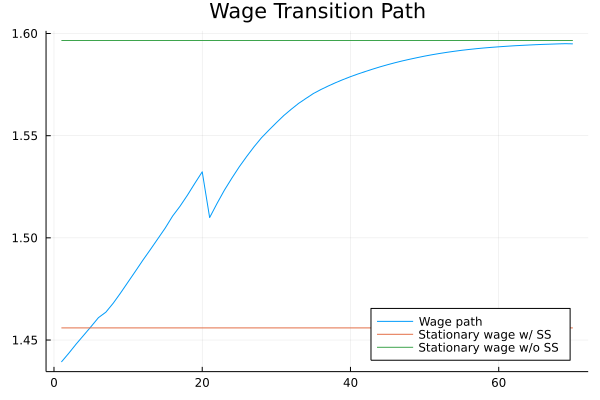
\includegraphics[width=.4\linewidth]{./julia/wage_path2.png}}
			\subfloat{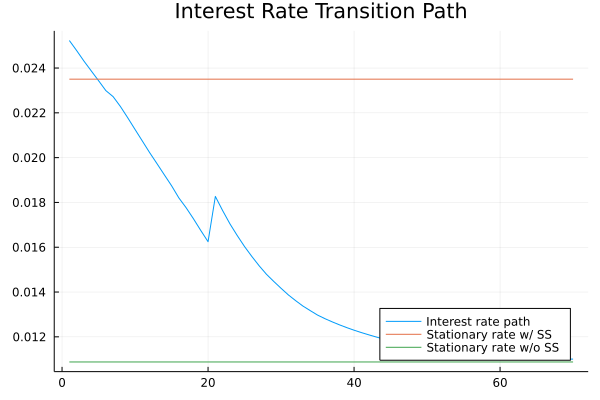
\includegraphics[width=.4\linewidth]{./julia/interest_rate_path2.png}}
		\end{figure}

		\begin{figure}[h]
			\centering
			\subfloat{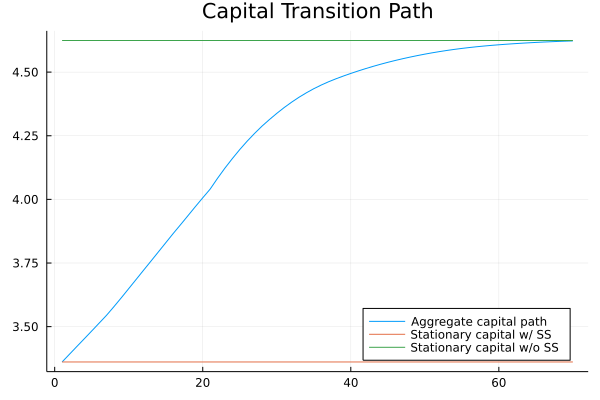
\includegraphics[width=.4\linewidth]{./julia/aggregate_capital_path2.png}}
			\subfloat{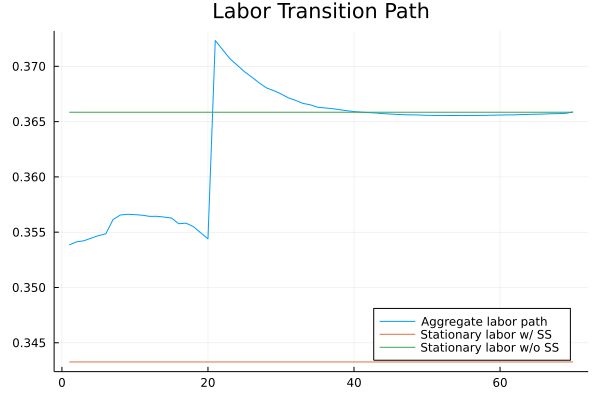
\includegraphics[width=.4\linewidth]{./julia/aggregate_labor_path2.png}}
		\end{figure}
	
	~\\
	The proportion of people who support the reform will substantially increase to $22.3\%$. Still, the majority of population will be against the reform.
		
	\begin{center}
	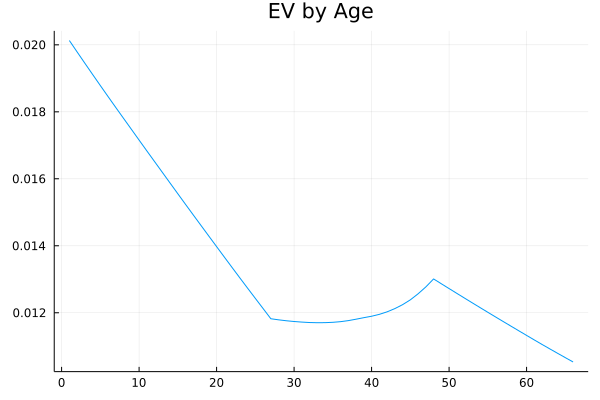
\includegraphics[width=.5\linewidth]{./julia/EV2.png}
	\end{center}
	
\end{itemize}
	
\end{document}